% Foliensatz: "AFu-Kurs nach DJ4UF" von DK0TU, Amateurfunkgruppe der TU Berlin
% Lizenz: CC BY-NC-SA 3.0 de (http://creativecommons.org/licenses/by-nc-sa/3.0/de/)
% Autoren: Sebastian Lange <dl7bst@dk0tu.de>
% Korrekturen: Lars Weiler <dc4lw@darc.de>

\documentclass[aspectratio=169]{beamer}

\usepackage[ngerman]{babel} % deutsche Worttrennung etc.
\usepackage[utf8]{inputenc} % UTF8 Text

\usepackage[super, comma, numbers, square, sort]{natbib}

\usepackage{hyperref}       % Hyperref Package für bessere Referenzen (todo)
\hypersetup{
	colorlinks=false,       %   false: boxed links; true: colored links
    %linkcolor=white,       %   color of internal links (change box color with linkbordercolor)
    citecolor=red,          %   color of links to bibliography
    filecolor=white,        %   color of file links
    urlcolor=blue           %   color of external links
}

\usepackage{multirow}
\usepackage{wasysym}  % Math Symbols like \permil
%\usepackage{colortbl}
%\usepackage{subscript}
%\usepackage{caption}
%\usepackage{setspace}
%\usepackage{xcolor}        % benutze CodeListe

% Footnote
%\usepackage{hanging}
%
%\setbeamertemplate{footnote}{%
%  \hangpara{2em}{1}%
%  \makebox[2em][l]{\insertfootnotemark}\footnotesize\insertfootnotetext\par%
%}


%\usepackage{pgf}
%\usepackage{tikz}
%\usetikzlibrary{arrows,automata}
%\usetikzlibrary{positioning}
%
%\tikzset{
%    state/.style={
%           rectangle,
%           rounded corners,
%           draw=black, very thick,
%           minimum height=2em,
%           minimum width=2pt,
%           inner sep=2pt,
%           text centered,
%           },
%}

%\usepackage{listings}
%\lstset{basicstyle=\small, numberstyle=\tiny, extendedchars=true, numbers=left, numbersep=5pt}
%\lstset{showtabs=false, showspaces=false, showstringspaces=false}
%%\lstset{backgroundcolor=\color{white!75!lightgray}, , frame=single}
%%\lstset{backgroundcolor=\color{white}}
%%\lstset{backgroundcolor=none}
%\lstset{keywordstyle=\color{blue!50!gray},  identifierstyle=\color{black}}
%\lstset{commentstyle=\color{green!50!gray}, stringstyle=\color{red!50!gray}}
%\lstset{language=C, fontadjust=true, tabsize=2, breaklines=true}
%\lstset{backgroundcolor=\color{white!75!lightgray}, caption=\lstname, frame=single}
%\lstset{emphstyle=\color{black}\fbox}
%
%% Keine "Listing:"-Caption
%\captionsetup{labelformat=empty,labelsep=none}
%
%% für mathematische Umgebungen
%\usepackage{amsmath,amsfonts,amssymb}
%
%\lstdefinestyle{Bash}{
%language=Bash,
%frame=single,
%rulecolor=\color{black},
%backgroundcolor=\color{gray!50},
%keywordstyle=\color{black},
%identifierstyle=,
%commentstyle=\color{black},
%stringstyle=\color{magenta!65!white},
%showstringspaces=false,
%basicstyle=\footnotesize\ttfamily\color{black},
%numbers=none,
%breaklines=true,
%captionpos=b
%}

%\usepackage{listings}
%
%\lstdefinestyle{basic}{
%    captionpos=t,%
%    basicstyle=\footnotesize\ttfamily,%
%    numberstyle=\tiny,%
%    numbers=left,%
%    stepnumber=1,%
%    frame=single,%
%    showspaces=false,%
%    showstringspaces=false,%
%    showtabs=false,%
%    %
%    keywordstyle=\color{blue},%
%    identifierstyle=,%
%    commentstyle=\color{gray},%
%    stringstyle=\color{magenta}%
%}



% fließende Boxen haben keinen Abstand
%\fboxsep0mm

% inkludiere Creative Commons Helper
%%%%%%%%%%%%%%%%%%%%%%%%%%%%%%%%%%%%%%%%%%%%%%%%%%%%%%%%%%%%%%%%
%% ccBeamer 0.1, 2007-07-02                                   %%
%% Written by Sebastian Pipping <webmaster@hartwork.org>      %%
%% ---------------------------------------------------------- %%
%% Licensed under Creative Commons Attribution-ShareAlike 3.0 %%
%% http://creativecommons.org/licenses/by-sa/3.0/             %%
%%%%%%%%%%%%%%%%%%%%%%%%%%%%%%%%%%%%%%%%%%%%%%%%%%%%%%%%%%%%%%%%


%% Images
\newcommand{\CcImageBy}[1]{%
	
\includegraphics[scale=#1]{texdata/creative_commons/cc_by_30.pdf}%
}
\newcommand{\CcImageCc}[1]{%
	
\includegraphics[scale=#1]{texdata/creative_commons/cc_cc_30.pdf}%
}
\newcommand{\CcImageDevNations}[1]{%
	
\includegraphics[scale=#1]{texdata/creative_commons/cc_dev_nations_30.pdf}%
}
\newcommand{\CcImageNc}[1]{%
	
\includegraphics[scale=#1]{texdata/creative_commons/cc_nc_30.pdf}%
}
\newcommand{\CcImageNd}[1]{%
	
\includegraphics[scale=#1]{texdata/creative_commons/cc_nd_30.pdf}%
}
\newcommand{\CcImagePd}[1]{%
	
\includegraphics[scale=#1]{texdata/creative_commons/cc_pd_30.pdf}%
}
\newcommand{\CcImageSa}[1]{%
	
\includegraphics[scale=#1]{texdata/creative_commons/cc_sa_30.pdf}%
}
\newcommand{\CcImageSampling}[1]{%
	
\includegraphics[scale=#1]{texdata/creative_commons/cc_sampling_30.pdf}%
}
\newcommand{\CcImageSamplingPlus}[1]{%
	
\includegraphics[scale=#1]{texdata/creative_commons/cc_sampling_plus_30.pdf}%
}


%% Groups
\newcommand{\CcGroupBy}[2]{% zoom, gap
	\CcImageCc{#1}\hspace*{#2}\CcImageBy{#1}%
}
\newcommand{\CcGroupByNc}[2]{% zoom, gap
	\CcImageCc{#1}\hspace*{#2}\CcImageBy{#1}\hspace*{#2}\CcImageNc{#1}%
}
\newcommand{\CcGroupByNcNd}[2]{% zoom, gap
	\CcImageCc{#1}\hspace*{#2}\CcImageBy{#1}\hspace*{#2}\CcImageNc{#1}\hspace*{#2}\CcImageNd{#1}%
}
\newcommand{\CcGroupByNcSa}[2]{% zoom, gap
	\CcImageCc{#1}\hspace*{#2}\CcImageBy{#1}\hspace*{#2}\CcImageNc{#1}\hspace*{#2}\CcImageSa{#1}%
}
\newcommand{\CcGroupByNd}[2]{% zoom, gap
	\CcImageCc{#1}\hspace*{#2}\CcImageBy{#1}\hspace*{#2}\CcImageNd{#1}%
}
\newcommand{\CcGroupBySa}[2]{% zoom, gap
	\CcImageCc{#1}\hspace*{#2}\CcImageBy{#1}\hspace*{#2}\CcImageSa{#1}%
}
\newcommand{\CcGroupDevNations}[2]{% zoom, gap
	\CcImageCc{#1}\hspace*{#2}\CcImageDevNations{#1}%
}
\newcommand{\CcGroupNcSampling}[2]{% zoom, gap
	\CcImageCc{#1}\hspace*{#2}\CcImageNc{#1}\hspace*{#2}\CcImageSampling{#1}%
}
\newcommand{\CcGroupPd}[1]{% zoom
	\CcImagePd{#1}%
}
\newcommand{\CcGroupSampling}[1]{% zoom
	\CcImageSampling{#1}%
}
\newcommand{\CcGroupSamplingPlus}[1]{% zoom
	\CcImageSamplingPlus{#1}%
}


%% Text
\newcommand{\CcLongnameBy}{Attribution}
\newcommand{\CcLongnameByNc}{Attribution-NonCommercial}
\newcommand{\CcLongnameByNcNd}{Attribution-NoDerivs}
\newcommand{\CcLongnameByNcSa}{Attribution-NonCommercial-ShareAlike}
\newcommand{\CcLongnameByNd}{Attribution-NoDerivs}
\newcommand{\CcLongnameBySa}{Attribution-ShareAlike}

\newcommand{\CcNote}[1]{% longname
	This work is licensed under the \textit{Creative Commons #1 3.0 License}.%
}


% generelles Thema auswählen
\usetheme{Goettingen} %Berlin spart ohne Sidebar allerdings angenehm Platz
% AnnArbor | Antibes | Bergen | Berkeley | Berlin | Boadilla | boxes | CambridgeUS | Copenhagen | Darmstadt | default | Dresden | Frankfurt | Goettingen | Hannover | Ilmenau | JuanLesPins | Luebeck | Madrid | Malmoe | Marburg | Montpellier | PaloAlto | Pittsburgh | Rochester | Singapore | Szeged | Warsaw

% Farben wählen
\usecolortheme{beetle}
% beaver | beetle | crane | default | dolphin | dove | fly | lily | orchid | rose | seagull | seahorse | sidebartab | structure | whale | wolverine

% Setze alle Farben auf Grau und Weiß
%\definecolor{craneorange}{RGB}{64,64,64}
%\definecolor{craneblue}{RGB}{255,255,255}

% Schriftart wählen
\usefonttheme{default}
% default | professionalfonts | serif | structurebold | structureitalicserif | structuresmallcapsserif

% Innere Themen(Kopf-, Fuß-, Sidebar usw)
%\useinnertheme{default}
\useinnertheme{circles}
% default | inmargin | rectangles | rounded | circles

% Äußere Themen (Anordnung der inneren, grenzen der Folien etc.)
\useoutertheme{infolines}
% default | infolines | miniframes | shadow | sidebar | smoothbars | smoothtree | split | tree

% Deaktiviere Navigations-Symbole ({} -> leer)
\setbeamertemplate{navigation symbols}{}
%\setbeamertemplate{navigation symbols}{\large \ifnum \insertframenumber <10 0\fi\insertframenumber/\inserttotalframenumber\vspace*{0.2ex}}

% Zeige ein Hintergrundbild
\setbeamertemplate{background canvas}{
        \hspace*{-2.0cm}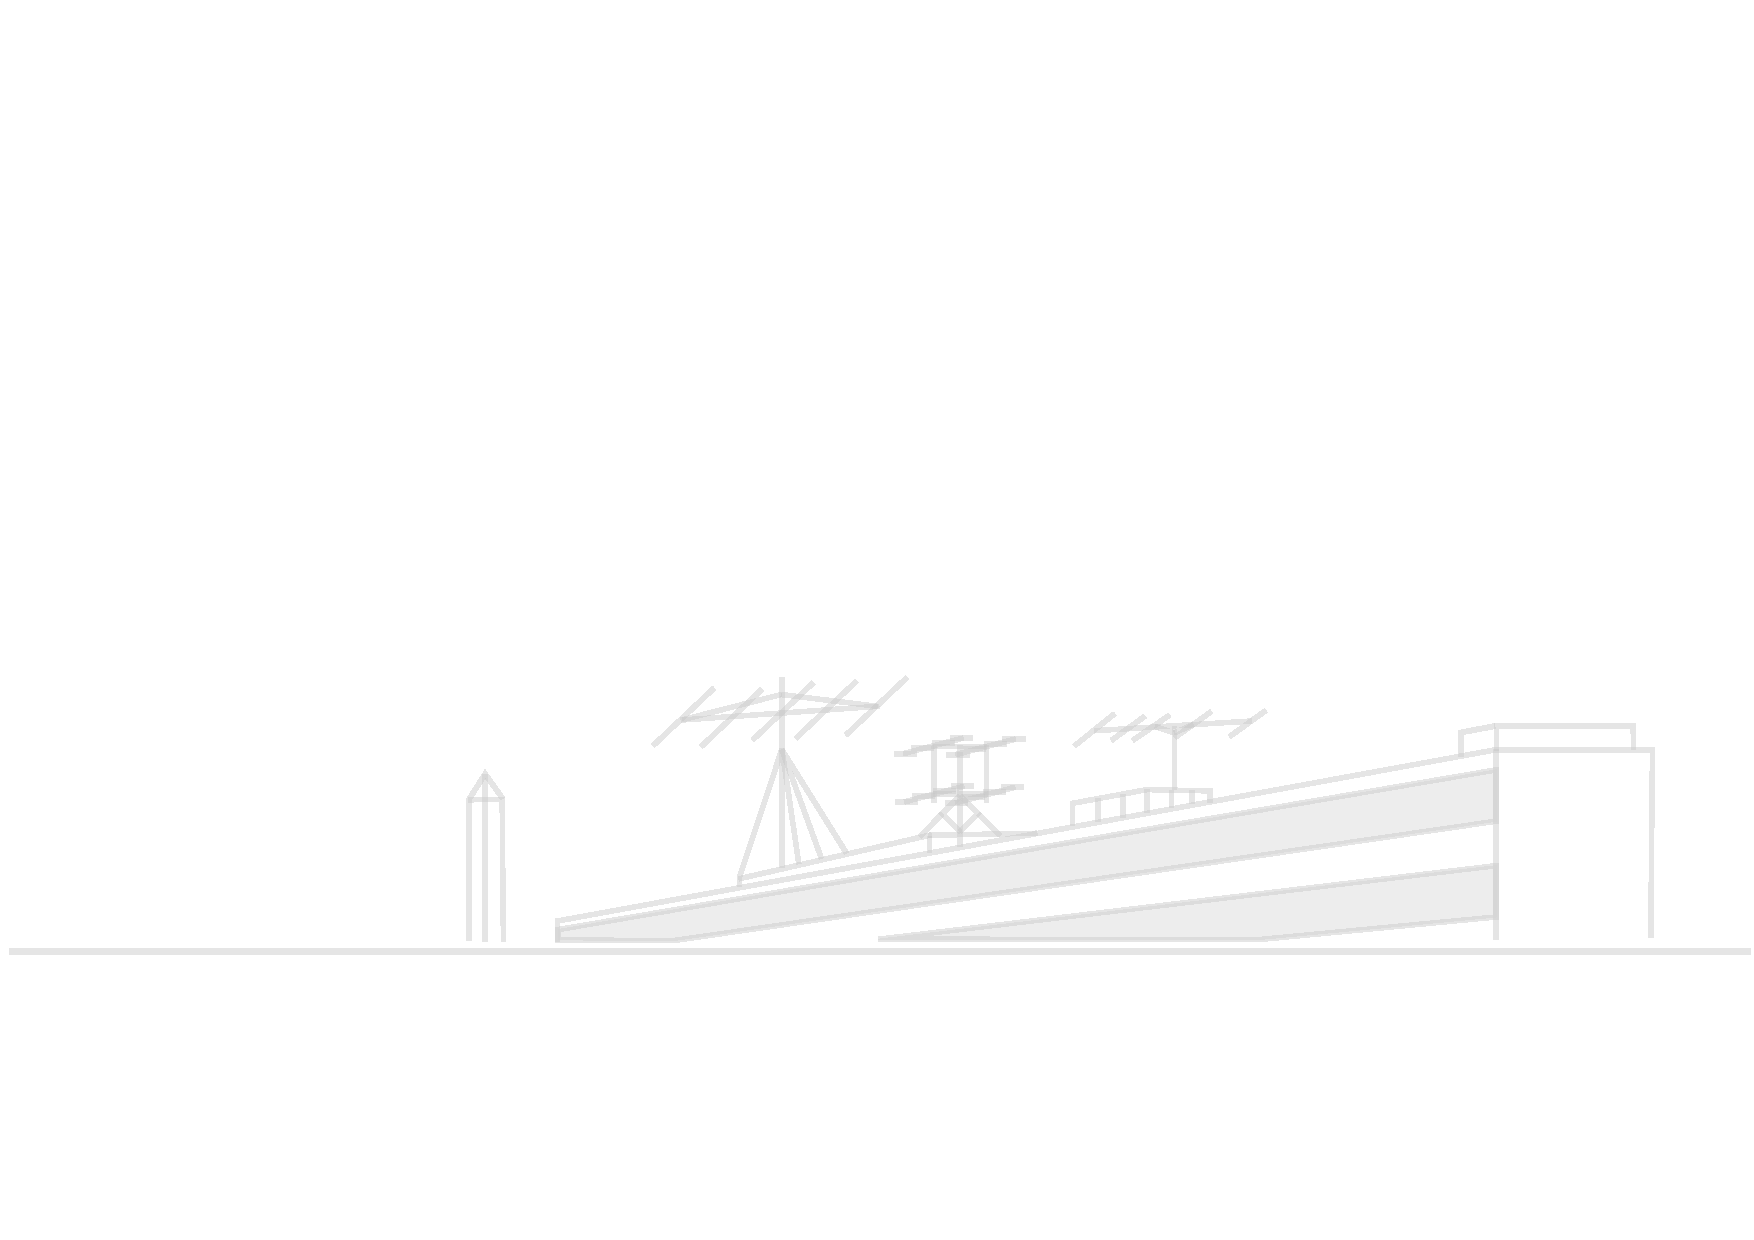
\includegraphics[width=17.8cm]{texdata/dk0tu_rooftop_background.pdf}
}

% Foliennummer einfügen
\setbeamertemplate{footline}[frame number]
%\setbeamertemplate{footline}{}

% Ändere das Zeichen vor jedem item
%\setbeamertemplate{itemize item}{\color{craneorange}$\blacktriangleright$}
%\setbeamertemplate{itemize subitem}{\color{craneorange}$\triangleright$}
%\setbeamertemplate{itemize subsubitem}{\color{craneorange}$\blacktriangleright$}

% Ändert die Blöcke 
\setbeamertemplate{blocks}[rounded][shadow=true]
% default | rounded [shadow=true|false]

%
% Eigene Kommandos
%

% Hack to get natbib and beamer working together. "The beamer user guide suggests
% that only the manual bibliography entry approach is supported"
% on some system it works out of the box, sometimes you need the hack :-(
% so check it --dl7bst
\ifdefined\newblock
    \relax
\else
    \newcommand{\newblock}{}
\fi

% \includedia command to generate png out of a dia file
% NEEDS installed dia and pdflatex option --shell-escape
\newcommand{\includedia}[1]{
    \immediate\write18{/usr/bin/dia #1.dia -e #1_diatmp.png -t png}
}

% RICHIG GROSSER FONT!
\newfont{\bigfont}{cmr10 at 144pt}
\newfont{\smallfont}{cmr10 at 8pt}

% Römische Ziffern
\makeatletter
\newcommand{\rmnum}[1]{\romannumeral #1}
\newcommand{\Rmnum}[1]{\expandafter\@slowromancap\romannumeral #1@}
\makeatother

% Schwarze Überschrift
%\setbeamercolor{frametitle}{fg=black}
%\setbeamercolor{title}{fg=black}

% Item- und Box-Farben
\definecolor{deepBlue}{HTML}{000066}
\setbeamercolor{itemize item}{fg=deepBlue}
\setbeamercolor{itemize subitem}{fg=deepBlue}
\setbeamercolor{description item}{fg=deepBlue}
\setbeamercolor{block title}{fg=deepBlue!100, bg=blue!15}
\setbeamercolor{block body}{fg=black, bg=blue!5}
\setbeamercolor{block title alerted}{fg=deepBlue, bg=red!75}
\setbeamercolor{block body alerted}{fg=black, bg=red!15}
\setbeamercolor*{block title example}{fg=blue!50, bg=blue!10}
\setbeamercolor*{block body example}{fg= blue, bg=blue!5}

%\setbeamercolor{section in head/foot}{parent=palette primary}
%\setbeamercolor{subsection in head/foot}{parent=palette secondary}
%\setbeamercolor{sidebar}{fg=darkblue,bg=yellow!90!orange}
%\setbeamercolor{title in sidebar}{fg=darkblue}
%\setbeamercolor{author in sidebar}{fg=darkblue}
%\setbeamercolor{section in sidebar}{fg=darkblue!10!black}
%\setbeamercolor{subsection in sidebar}{fg=darkblue!50!black}

% Titlepage Infos
\title{AFu-Kurs nach DJ4UF}
\author[DKØTU]{DKØTU\\ \footnotesize{Amateurfunkgruppe der TU Berlin}}
\institute[DKØTU]{\url{http://www.dk0tu.de} }

% PDF-Eigenschaften
\subject{DK0TU-Amateurfunkkurs nach DJ4UF}
\keywords{Amateurfunk Kurs HAM Radio Course CC-BY-NC-SA OpenSource TU Berlin DK0TU}

\subtitle{Betriebstechnik/Vorschriften 03: \\
  Der ``Q-Schlüssel''              \\[2em]}
\date{Stand 18.09.2017}
 \begin{document}

\begin{frame}
    \titlepage
    \vfill
    \begin{center}
        \ccbyncsaeu\\
        {\tiny This work is licensed under the \em{Creative Commons Attribution-NonCommercial-ShareAlike 3.0 License}.}\\[0.5ex]
         \tiny Amateurfunkgruppe der Technische Universität Berlin (AfuTUB), DKØTU
         %\includegraphics[scale=0.5]{img/DK0TU_Logo.pdf}
    \end{center}
\end{frame}


\section*{Einleitung}

\begin{frame}
  \frametitle{Einleitung / Q Code}
  \begin{center}
    \Large{Was ist das?} \\
    \Large{Kennt ihr ggf. welche?}
  \end{center}
\end{frame}

\begin{frame}
  \frametitle{Einleitung / Q Code}

  Bekannt aus Film und Fernsehen: \emph{QAM} $--\cdot-$ $\cdot-$ $--$ \\[2em]

  Ursprung: Seit 1912 organisationsübergreifende Vereinfachung von Nachrichten
  in Morsetelegrafie, eingeführt durch \emph{International Radiotelegraph
  Convention}.\footnote{\tiny Heute geregelt durch die Radio Regulations (RR)}
  \\[2em]

  Heute $>$250 Schlüssel:

  \begin{itemize}
    \item QAA bis QNZ: Flugfunkdienst
    \item QOA bis QQZ: Seefunkdienst
    \item QRA bis QUZ: alle Funkdienste
    \item QVA bis QZZ: andere, teilw. militärisch
  \end{itemize}

\end{frame}

\section*{Anwendung}

\begin{frame}
  \frametitle{Q Code / Verwendung}

  \begin{itemize}
    \item außer im AFu heute kaum noch genutzt
    \item Verwendung in der Morsetelegrafie \\
      (umgangssprachlich teilw. im Sprechfunk)
    \item Fragen einfach durch angehängtes Fragezeichen
    \item beliebige Ergänzungen durch Ziffern (1..5), Zahlen, Orte, Rufzeichen, \ldots
    \item Uhrzeiten grundsätzlich in UTC
      \footnote{\tiny Universal Time, Coordinated}
  \end{itemize}

\end{frame}

\begin{frame}
  \frametitle{Q Code / Beispiele}

  \only<1>{
  \begin{exampleblock}{Wie lautet das Rufzeichen?}
    \emph{QRZ?}
  \end{exampleblock}
  }

  \only<2>{
  \begin{exampleblock}{Soll ich die Sendeleistung verringern?}
    \emph{QRP?}
  \end{exampleblock}
  }

  \only<3>{
  \begin{exampleblock}{Mein Standort ist Berlin.}
    \emph{QTH Berlin}
  \end{exampleblock}
  }

  \only<4>{
  \begin{exampleblock}{Ich werde stark durch eine andere Station gestört.}
    \emph{QRM 4}
  \end{exampleblock}
  }

  \only<5>{
  \begin{block}{Q-Codes teils beliebige Buchstabengruppen}
    Es gibt aber \emph{Eselsbrücken}
  \end{block}
  }
\end{frame}



\begin{frame}
  \frametitle{(prüfungsrelevante) Q Codes / Amateurfunk}

  \begin{center}
    \scriptsize
    \only<1>{
    \begin{tabular}{lp{3cm}|lp{3cm}|p{3cm}}\hline
      Q   & Bedeutung & Q?   & Bedeutung & Eselsbrücke \\ \hline \hline
      QRA & Name der Station & QRA? & Wie ist der Name der Station? & \textbf{A}nrede \\
      QRG & Frequenz & QRG? & Wie ist die Frequenz? & \textbf{G}enaue Frequenz \\
      QRK & Lesbarkeit der Zeichen in RST-Stufen 1\ldots5 & QRK? & Wie hören Sie mich? & \\
      QRL & Operator beschäftigt & QRL? & Sind Sie beschäftigt? & \textbf{R}eal-\textbf{L}ife \\
      QRM & Gestört in Stufen 1\ldots5 & QRM? & Werden Sie gestört? & \textbf{R}eceive \textbf{M}ist \\
      QRN & Atmosphärische Störung in Stufen 1\ldots5 & QRN? & Haben Sie atmosphärische Störungen? & \textbf{N}oise / \textbf{N}atural \\
      QRP & Sendeleistung verringern & QRP? & Soll ich die Sendeleistung verringern? & \textbf{R}educe \textbf{P}ower \\
      QRO & Sendeleistung erhöhen & QRO? & Soll ich die Sendeleistung erhöhen? & Gegenteil von QRP \\
      QRX & Ich rufe Sie wieder um \ldots Uhr & QRX? & Wann rufen Sie mich wieder? & \\
      QRT & Übermittlung einstellen & QRT? & Soll ich die Übermittlung einstellen? & \textbf{T}erminate \\
    \end{tabular}
    }

    \only<2>{
    \begin{tabular}{lp{3cm}lp{3cm}p{2cm}}\hline
      Q   & Bedeutung & Q?   & Bedeutung & Eselsbrücke \\ \hline \hline
      QRV & Ich bin bereit & QRV? & Sind Sie bereit? & \textbf{V}erkehrsbereit \\
      QRZ & Sie werden von \ldots / auf \ldots gerufen & QRZ? & Von wem werde ich gerufen? & \\
      QSB & Signalstärke schwankt (Fading) & QSB? & Schwankt die Signalstärke? & \\
      QSL & Empfangsbestätigung & QSL? & Können Sie mir eine Empfangsbestätigung geben? & \\
      QTH & Standort & QTH? & Wie ist Ihr Standort? & \textbf{H}ome \\
      QSY & Frequenzwechsel auf \ldots & QSY? & Soll ich zum Senden auf eine andere Frequenz gehen? & \textbf{S}hift Frequenc\textbf{y}\\
      QSO & Funk-Verbindung / Gespräch & & & \\
    \end{tabular}
    }
  \end{center}
\end{frame}

\begin{frame}
  \frametitle{Noch mehr Beispiele}

  \only<1-2>{
  \begin{exampleblock}{QRX 1500 UTC}
    \only<1>{\vspace{1em}}
    \only<2>{Pause bis 15 Uhr UTC.}
  \end{exampleblock}
  }

  \only<3-4>{
  \begin{exampleblock}{QRX 5 min}
    \only<3>{\vspace{1em}}
    \only<4>{Pause für 5 Minuten.}
  \end{exampleblock}
  }

  \only<5-6>{
  \begin{exampleblock}{QRP?}
    \only<5>{\vspace{1em}}
    \only<6>{Können Sie die Sendeleistung verringern?}
  \end{exampleblock}
  }

  \only<7-8>{
  \begin{exampleblock}{QTH Essen}
    \only<7>{\vspace{1em}}
    \only<8>{Mein Standort ist Essen.}
  \end{exampleblock}
  }

  \only<9-10>{
  \begin{exampleblock}{tnx fer qso}
    \only<9>{\vspace{1em}}
    \only<10>{Danke für das Funkgespräch}
  \end{exampleblock}
  }
\end{frame}

\section*{Lernhilfen}

\begin{frame}
  \frametitle{Lernhilfen}

  Baut euch am Anfang möglichst \emph{Eselsbrücken}. Am Besten selbst
  ausdenken, aber Anregungen findet man auch bei anderen HAMs, z.B. hier: \\[2em]

  \ExternalLink \url{http://www.funkwelle.com/amateurfunk/q-schluessel-fuer-amateurfunkpruefung.html}

\end{frame}

\begin{frame}
  \begin{alertblock}{Hausaufgabe}
    Relevante Q-Gruppen für die Prüfung anschauen: Prüfungsfragen ``Betriebliche Kenntnisse'' Kapitel 2.2.2 ``Q-Schlüssel'' (BB201--BB209).
  \end{alertblock}
\end{frame}

\section*{Referenzen}

\begin{frame}
  \frametitle{Referenzen/Links}

  \footnotesize
  \begin{itemize}
    \item Moltrecht B/V 03: \\
      \url{https://www.darc.de/der-club/referate/ajw/lehrgang-bv/bv03/}
    \item Wikipedia DE: \\
      \url{http://de.wikipedia.org/wiki/Q-Schl\%C3\%BCssel}
    \item Wikipedia EN: \\
      \url{http://en.wikipedia.org/wiki/Q_code}
    \item List of Q-codes: \\
      \url{http://www.kloth.net/radio/qcodes.php}
  \end{itemize}

\end{frame}

% Hier könnte noch eine Kontaktfolie stehen

\end{document}

